\documentclass{article}

\usepackage[utf8]{inputenc}
\usepackage{graphicx}
\usepackage{amsmath}
\usepackage{amsfonts}
\usepackage{amssymb}
\usepackage{comment}
\usepackage{gensymb}
\usepackage{geometry}
\usepackage{float}
\usepackage{caption}
\usepackage{subcaption}
\usepackage{listings}
\usepackage{enumitem}
\usepackage{fontspec}
\usepackage{xcolor}

\setmonofont{JetBrainsMonoNerdFont-Regular.ttf}[Path=./]

% Catppuccin Macchiato color scheme
\definecolor{ctp-macchiato-rosewater}{HTML}{f4dbd6}
\definecolor{ctp-macchiato-flamingo}{HTML}{f0c6c6}
\definecolor{ctp-macchiato-pink}{HTML}{f5bde6}
\definecolor{ctp-macchiato-mauve}{HTML}{c6a0f6}
\definecolor{ctp-macchiato-red}{HTML}{ed8796}
\definecolor{ctp-macchiato-maroon}{HTML}{ee99a0}
\definecolor{ctp-macchiato-peach}{HTML}{f5a97f}
\definecolor{ctp-macchiato-yellow}{HTML}{eed49f}
\definecolor{ctp-macchiato-green}{HTML}{a6da95}
\definecolor{ctp-macchiato-teal}{HTML}{8bd5ca}
\definecolor{ctp-macchiato-sky}{HTML}{91d7e3}
\definecolor{ctp-macchiato-sapphire}{HTML}{7dc4e4}
\definecolor{ctp-macchiato-blue}{HTML}{8aadf4}
\definecolor{ctp-macchiato-lavender}{HTML}{b7bdf8}
\definecolor{ctp-macchiato-text}{HTML}{cad3f5}
\definecolor{ctp-macchiato-subtext1}{HTML}{b8c0e0}
\definecolor{ctp-macchiato-subtext0}{HTML}{a5adcb}
\definecolor{ctp-macchiato-overlay2}{HTML}{939ab7}
\definecolor{ctp-macchiato-overlay1}{HTML}{8087a2}
\definecolor{ctp-macchiato-overlay0}{HTML}{6e738d}
\definecolor{ctp-macchiato-surface2}{HTML}{5b6078}
\definecolor{ctp-macchiato-surface1}{HTML}{494d64}
\definecolor{ctp-macchiato-surface0}{HTML}{363a4f}
\definecolor{ctp-macchiato-base}{HTML}{24273a}
\definecolor{ctp-macchiato-mantle}{HTML}{1e2030}
\definecolor{ctp-macchiato-crust}{HTML}{181926}

\lstset{
    basicstyle=\ttfamily\color{ctp-macchiato-text},
    backgroundcolor=\color{ctp-macchiato-base},
    commentstyle=\color{ctp-macchiato-surface1},
    keywordstyle=\color{ctp-macchiato-mauve},
    stringstyle=\color{ctp-macchiato-green},
    identifierstyle=\color{ctp-macchiato-blue},
    frame=single,
    rulecolor=\color{ctp-macchiato-base},
    breaklines=true,
    breakatwhitespace=true,
    breakautoindent=true,
    showspaces=false,
    showstringspaces=false,
    showtabs=false,
    tabsize=4,
    captionpos=b,
    belowskip=1em,
    belowcaptionskip=2em
}

\lstdefinelanguage{myassembly}{
    basicstyle=\ttfamily\color{ctp-macchiato-text},
    backgroundcolor=\color{ctp-macchiato-base},
    commentstyle=\color{ctp-macchiato-surface1},
    keywordstyle=\color{ctp-macchiato-mauve},
    stringstyle=\color{ctp-macchiato-green},
    identifierstyle=\color{ctp-macchiato-blue},
    frame=single,
    rulecolor=\color{ctp-macchiato-base},
    breaklines=true,
    breakatwhitespace=true,
    breakautoindent=true,
    showspaces=false,
    showstringspaces=false,
    showtabs=false,
    tabsize=4,
    captionpos=b,
    belowskip=1em,
    belowcaptionskip=2em,
    % escapeinside={%}{)},
    morecomment=[l]{;},
    morestring=[b]",
    morekeywords={irmovq, rrmovq, mrmovq, rmmovq, pushq, popq, nop, halt, mov, add, sub, mul, div, cmp, jmp, je, jne, jg, jge, jl, jle, push, pop, call, ret, lea, xor, or, and, not, test},
    sensitive=false,
    upquote=true,
}

\geometry{a4paper, margin=1in}

\title{CSCE 312 Lab 6 - Term Project}
\author{Rita Hernandez Guerrero, Kevin Lei}

\date{May 2, 2024}

\begin{document}

\maketitle

\section{Y86 Instruction Set Architecture}
The circuit for the Y86 Instruction Set Architecture was implemented through Logisim. 
The circuit has five main subcircuits: the Fetch stage, the Decode and Write Back stage, the Execute stage, the Memory stage, and the PC Update stage.

\begin{figure}[H]
    \centering
    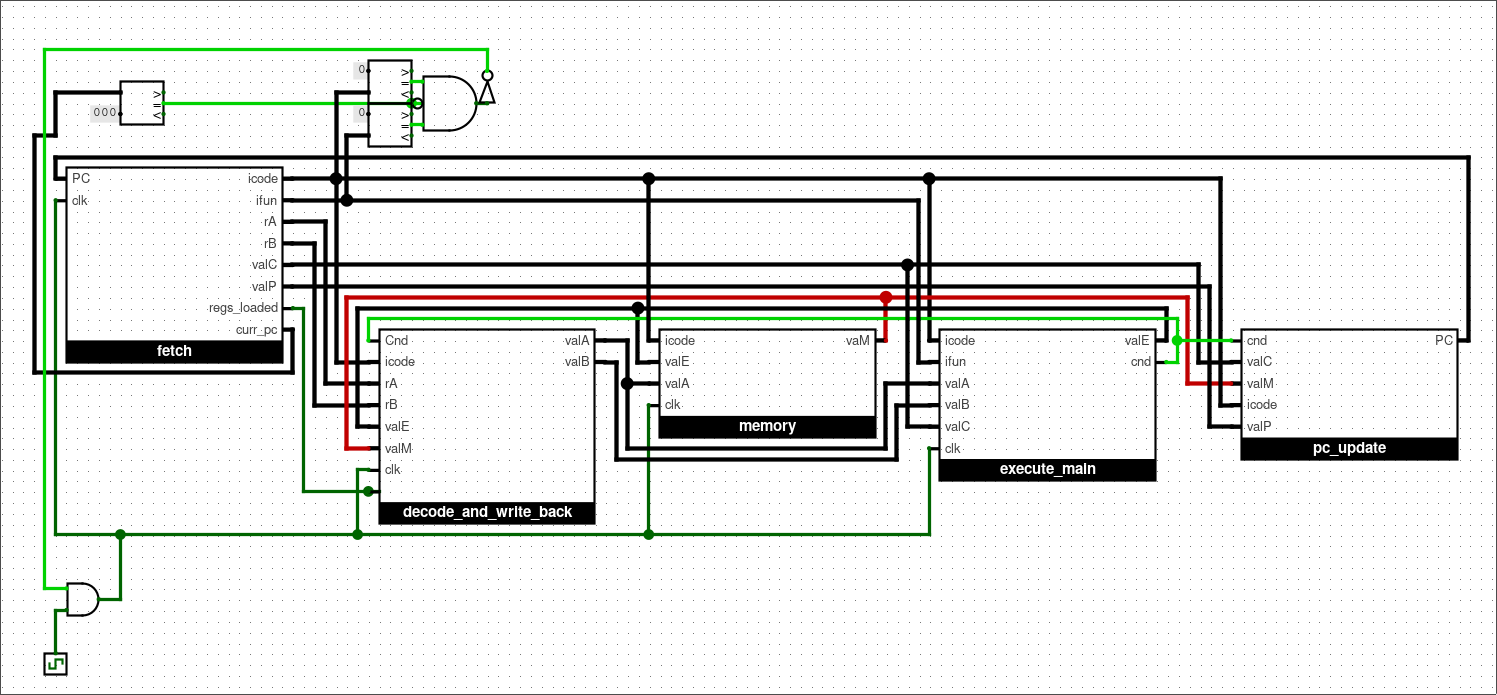
\includegraphics[width=0.8\textwidth]{./images/main_circuit.png}
    \caption{Main circuit for the Y86 ISA}
\end{figure}

\begin{figure}[H]
    \centering
    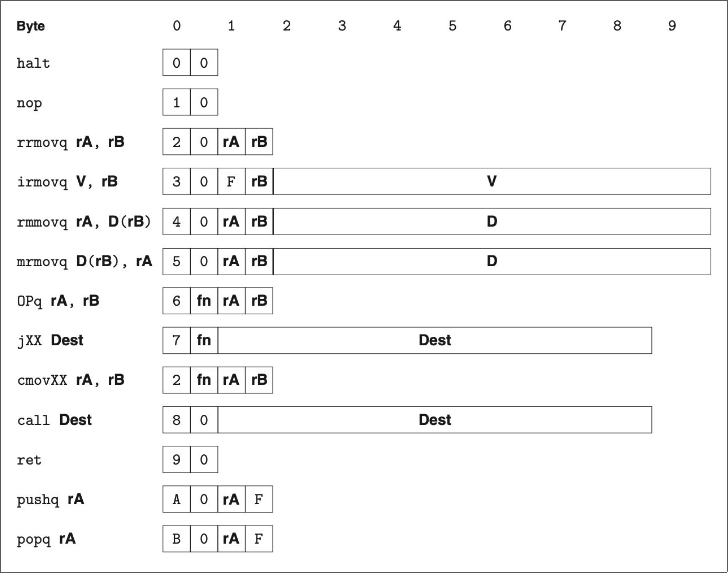
\includegraphics[width=0.7\textwidth]{./images/instructions.png}
    \caption{Instruction format}
\end{figure}
\newpage
\begin{figure}[H]
    \centering
    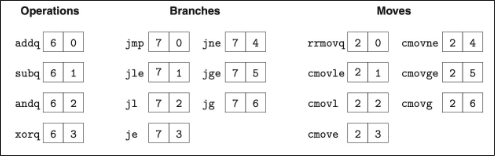
\includegraphics[width=0.7\textwidth]{./images/sub_instructions.png}
    \caption{Function specific instructions}
\end{figure}

\subsection{Fetch Stage}
In the Fetch stage, the instruction memory is implemented. 
The Fetch stage reads 10 bytes from memory at a time and the address of the first byte is stored in the PC (program counter). 
Then the stage produces meaningful data and control signals from the instruction for later stages. 
The Split module divides instruction byte into icode and ifun. 
The Align module gets fields for rA (register A), rB (register B), and valC. 
valC is the value constant which represents the immediate data that may be used for certain instructions (loading into a register or calculating in an arithmetic operation). 

\begin{figure}[H]
    \centering
    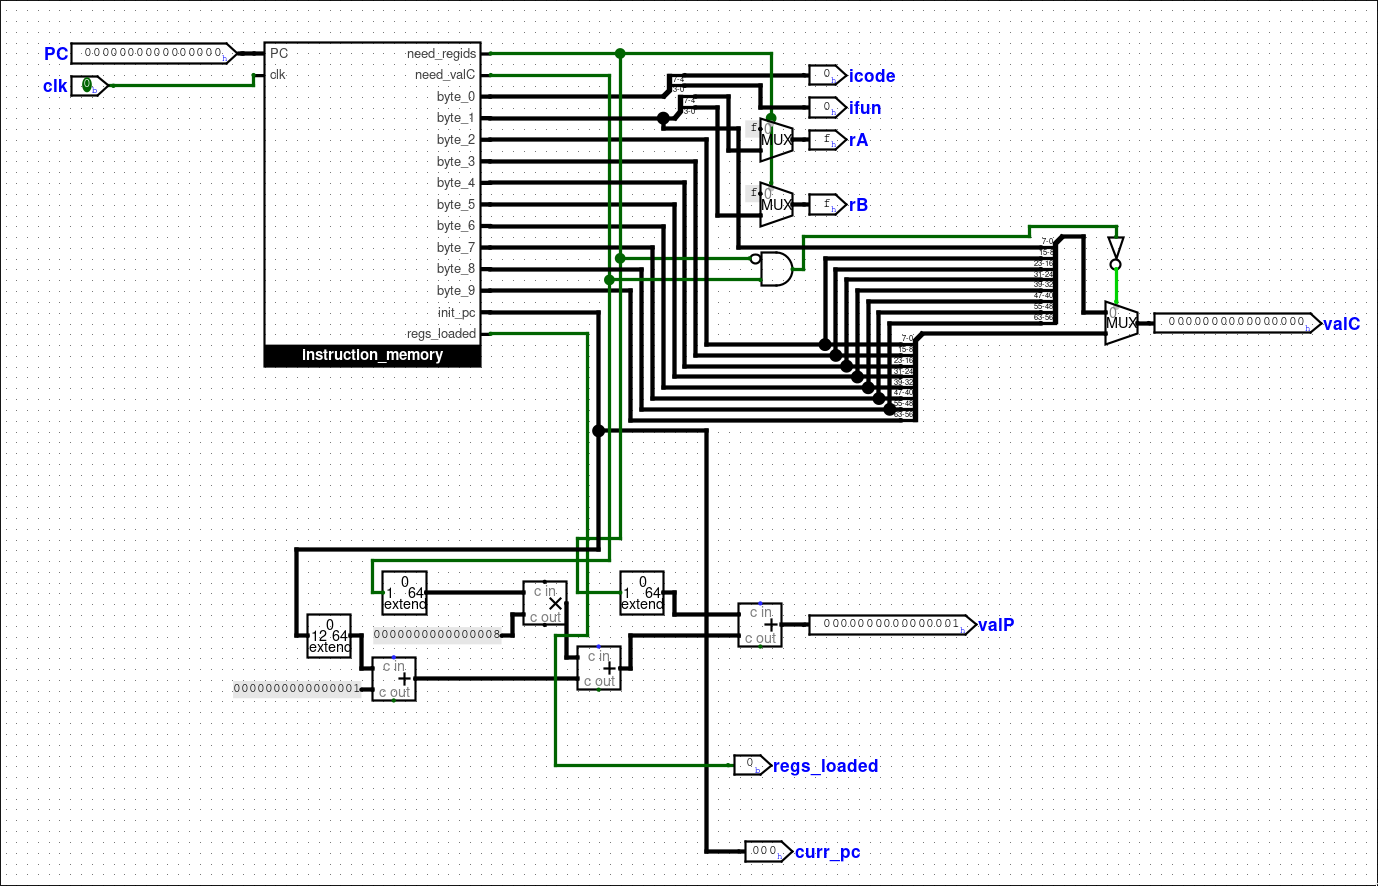
\includegraphics[width=0.8\textwidth]{./images/fetch.png}
    \caption{Fetch stage}
\end{figure}

Within the instruction memory, a 4kx8 RAM is used to read the instruction memory. 
The total size is 4KB because of the 12-bit address width and the 8-bit of data bit width that are both read. 
The value from the RAM is then broken up into 10 different register files, each register file representing a byte of the instruction memory line. 
A counter is set up to make sure that each line of the instruction memory is read. 

\begin{figure}[H]
    \centering
    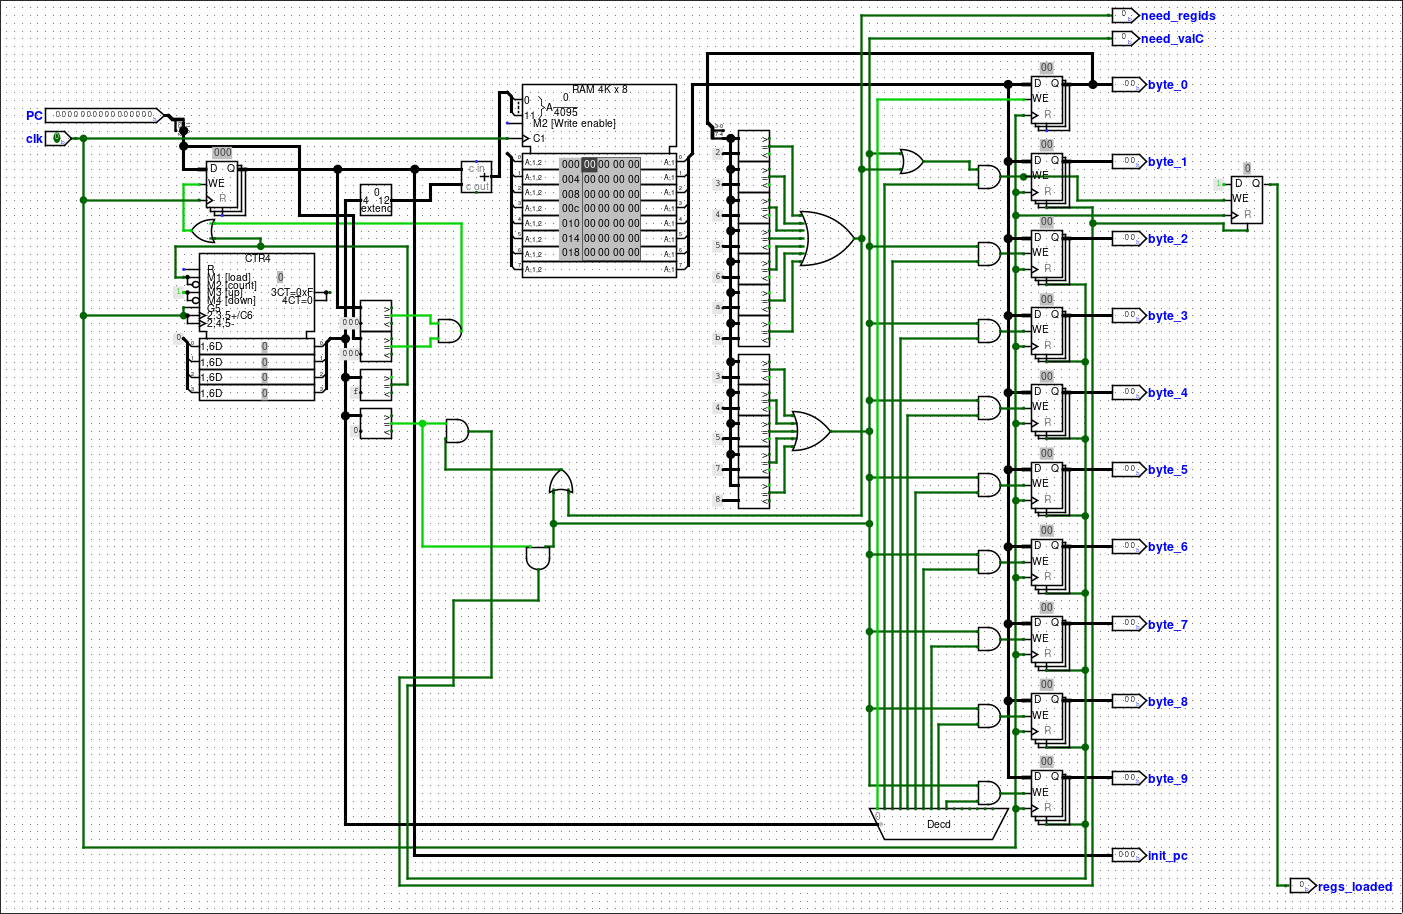
\includegraphics[width=0.8\textwidth]{./images/instruction_memory.png}
    \caption{Instruction memory}
\end{figure}

\subsection{Decode and Write Back Stage}

Data is read from register files in the decode stage. 
The register file has two ports for reads. 
One being srcA and the other being represented as srcB. 
dstE, dstM are the outputs and are the write port addresses. 
Register ids are selected by the instruction code (icode). 
If the fetched instruction does not have to read/write register, a default value of 0xF is selected. 
The module also takes into account the Cnd value which indicates whether or not a conditional move is needed. 
The Cnd value is computed from the Execute stage.

\begin{figure}[H]
    \centering
    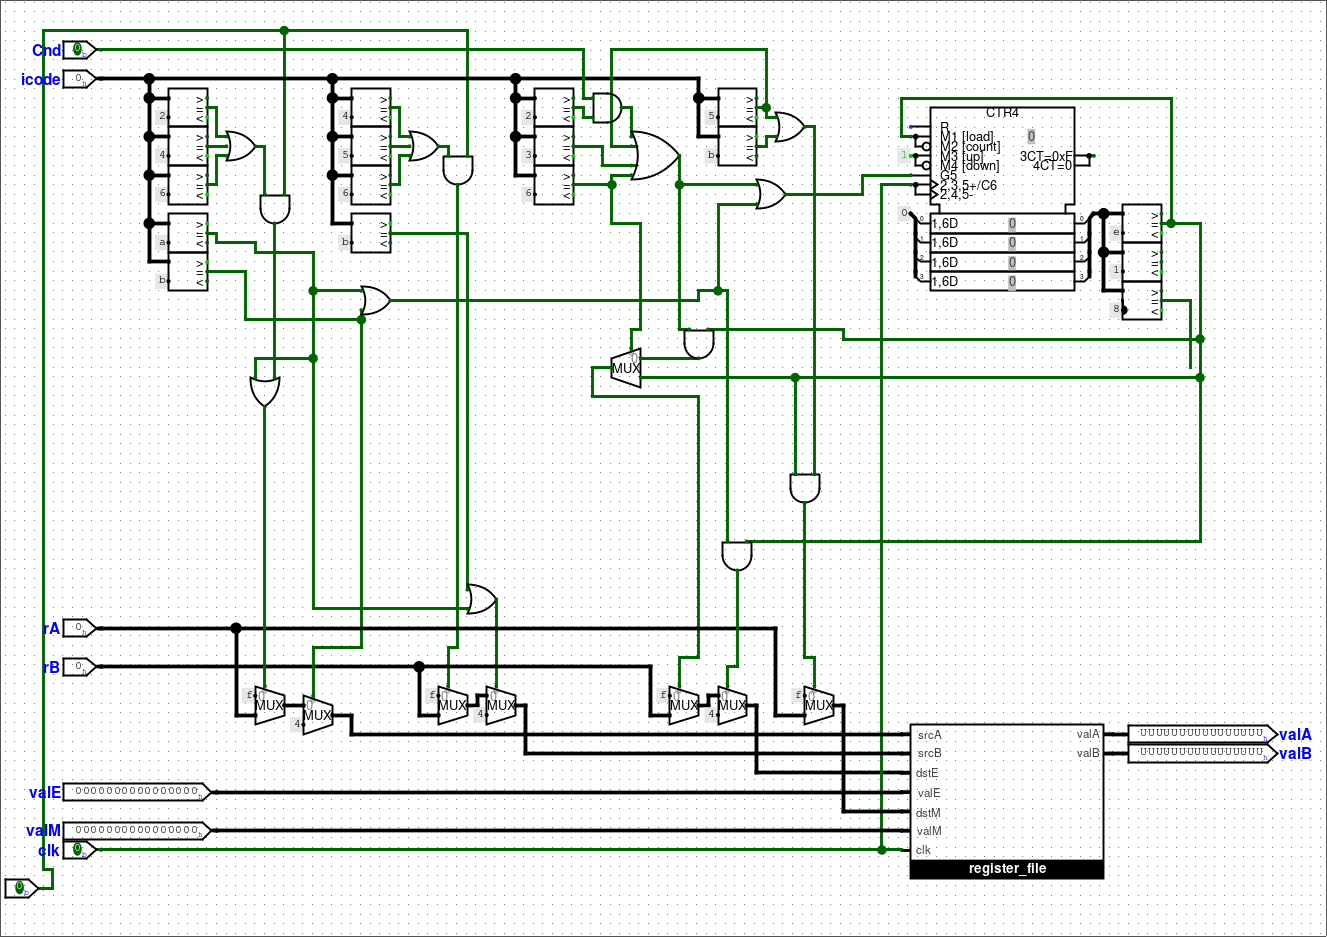
\includegraphics[width=0.8\textwidth]{./images/decode_write_back.png}
    \caption{Decode and Write Back stage}
\end{figure}

Within the Decode and Write Back stage, a register file component is implemented to read and write data from the 15 registers.

\begin{figure}[H]
    \centering
    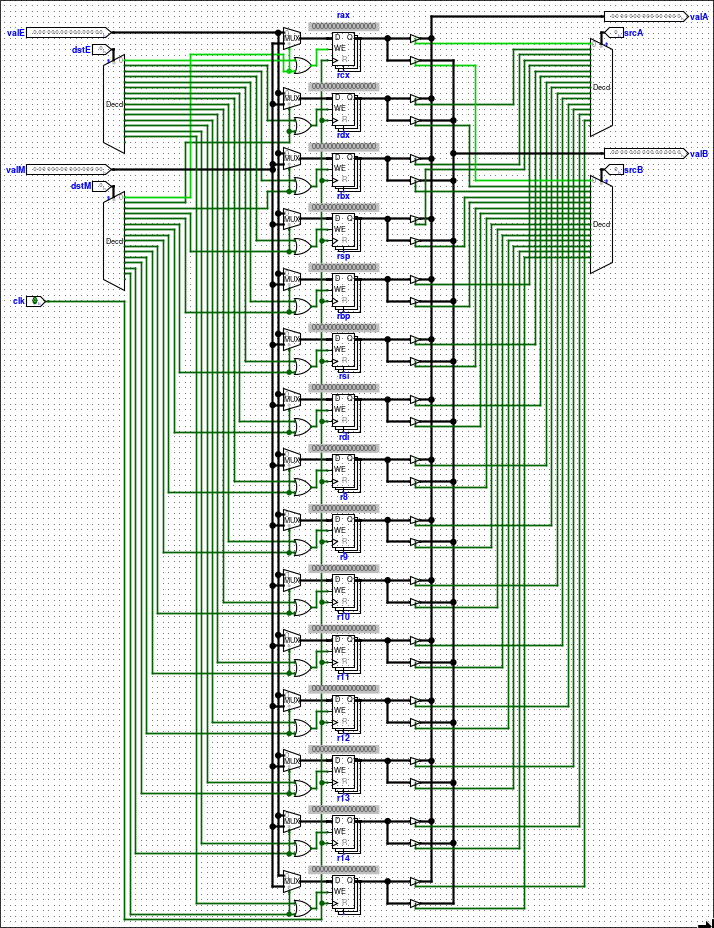
\includegraphics[width=0.8\textwidth]{./images/register_file.png}
    \caption{Register file}
\end{figure}

\subsection{Execute Stage}

The Execution stage mainly surrounds the Arithmetic Logic Unit (ALU) performing the four operations (addq, subq, andq, and xorq). 
A condition code is also calculated in a form of (Zero Flag/Sign Flag/Overflow Flag). 
The Condition Code (CC) module lets the CC store the last condition code. 
The SetCC module generates a signal to store CC. It is set if the icode is 6 (OPq). 
The signal of Cond is used by jXX in NewPC, cmovXX in Write Back stage. 
ALU\_fun determines the operation that must be operated by the ALU. 
ALU\_A and ALU\_B compute the inputs for the ALU. 

\begin{figure}[H]
    \centering
    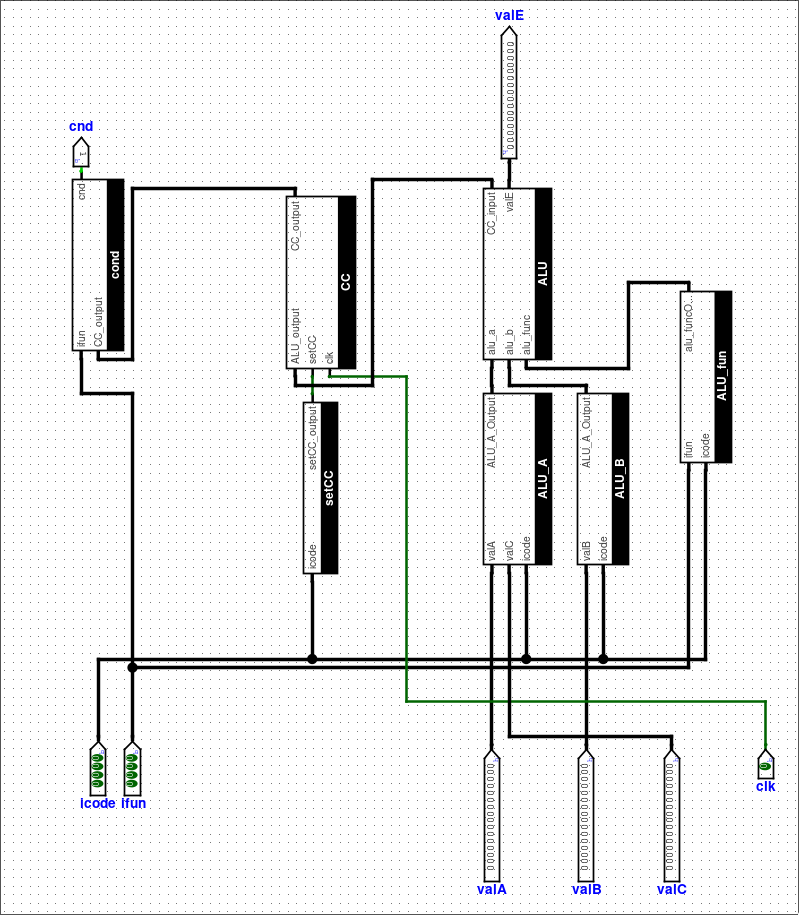
\includegraphics[width=0.8\textwidth]{./images/execute.png}
    \caption{Execute stage}
\end{figure}

\begin{figure}[H]
    \centering
    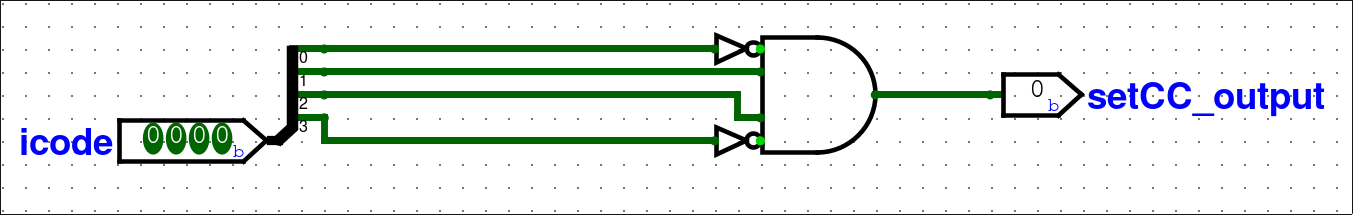
\includegraphics[width=0.8\textwidth]{./images/set_cc.png}
    \caption{Set Condition Code module}
\end{figure}

As mentioned above, ALU\_A and ALU\_B both determine the inputs of the ALU depending on the instruction code given. 
For example, the instruction code (icode) determines if ALU\_A's output will be either valA, valC, 8 or -8 through a 16x1 multiplexer. 

\begin{figure}[H]
    \centering
    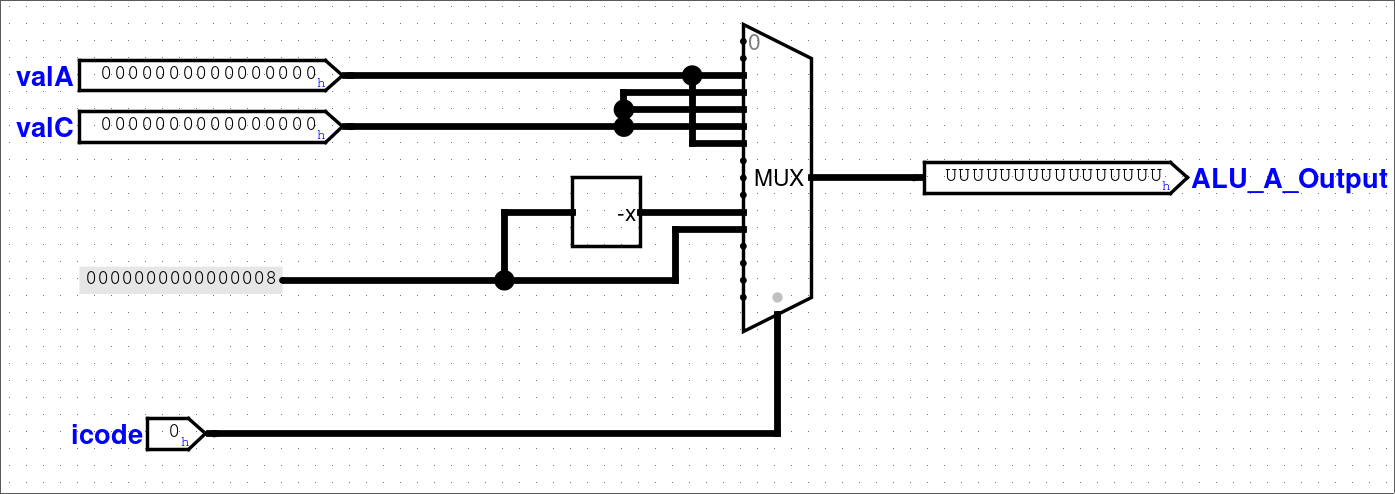
\includegraphics[width=0.8\textwidth]{./images/alu_a.png}
    \caption{ALU\_A module}
\end{figure}

Likewise, the output for ALU\_B was derived from a 16x1 multiplexer that chose from either 0 or valB, depending on the instruction code. 

\begin{figure}[H]
    \centering
    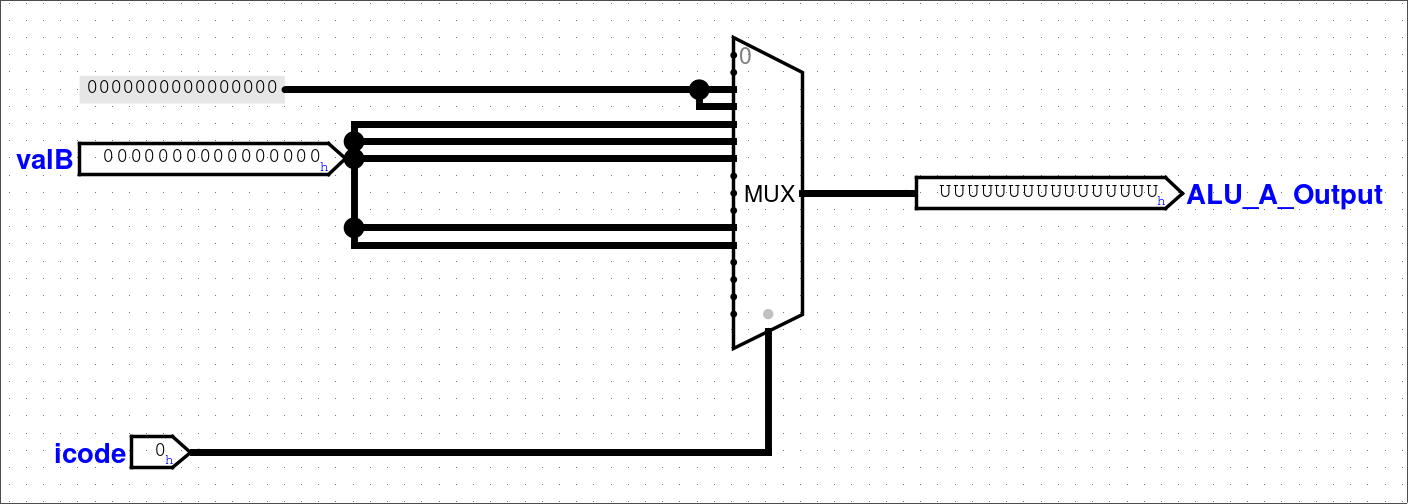
\includegraphics[width=0.8\textwidth]{./images/alu_b.png}
    \caption{ALU\_B module}
\end{figure}

To find out which function the ALU has to perform, a 16x1 multiplexer uses the instruction code to choose between 0 (addition) or other functions determined by ifun (the instruction function).  

\begin{figure}[H]
    \centering
    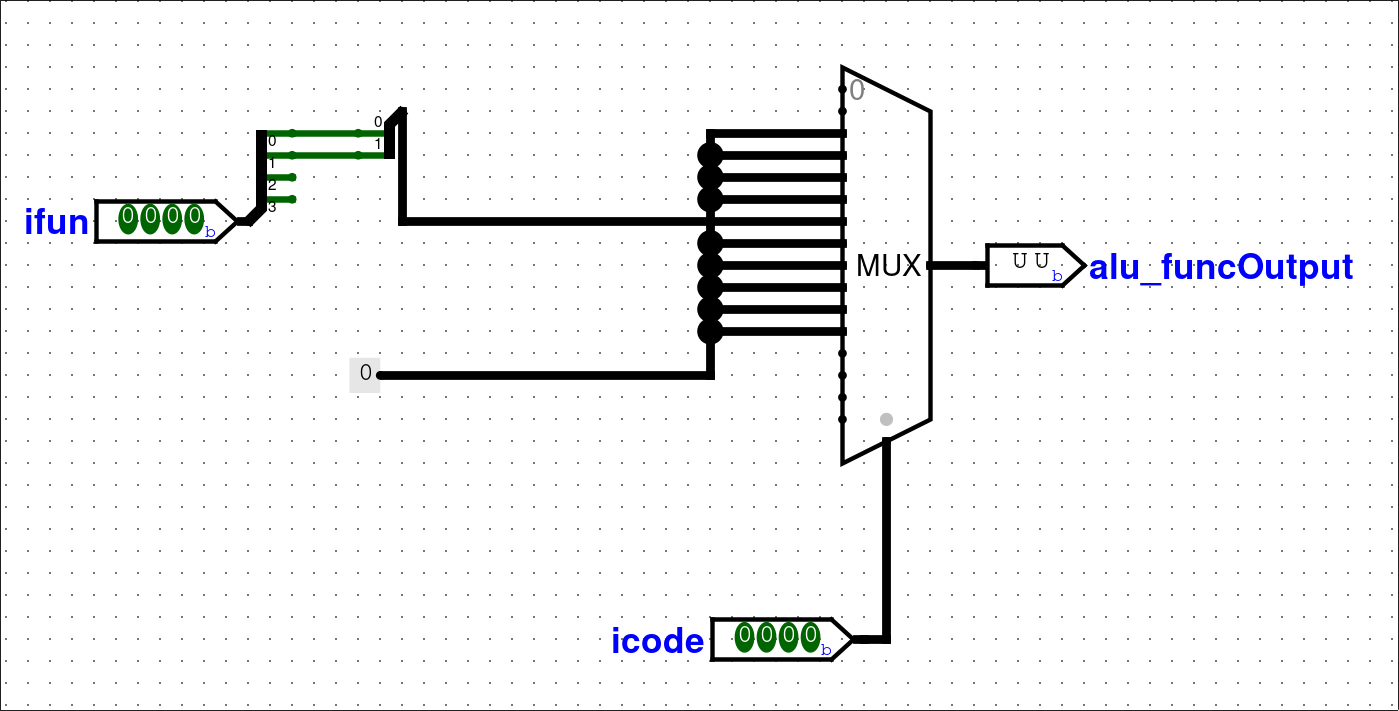
\includegraphics[width=0.8\textwidth]{./images/alu_fun.png}
    \caption{ALU\_fun module}
\end{figure}

The condition module sets the condition flag off (cnd) depending on the condition code found by the ALU and the instruction function being read. 
For example, if the instruction function were jl (ifun = 2), the expected condition code would be an input of 011 (ZF/SF/OF). 
AND gates are set in place to make sure both inputs are met. 
If both inputs meet the requirement, then cnd will output 1. 

\begin{figure}[H]
    \centering
    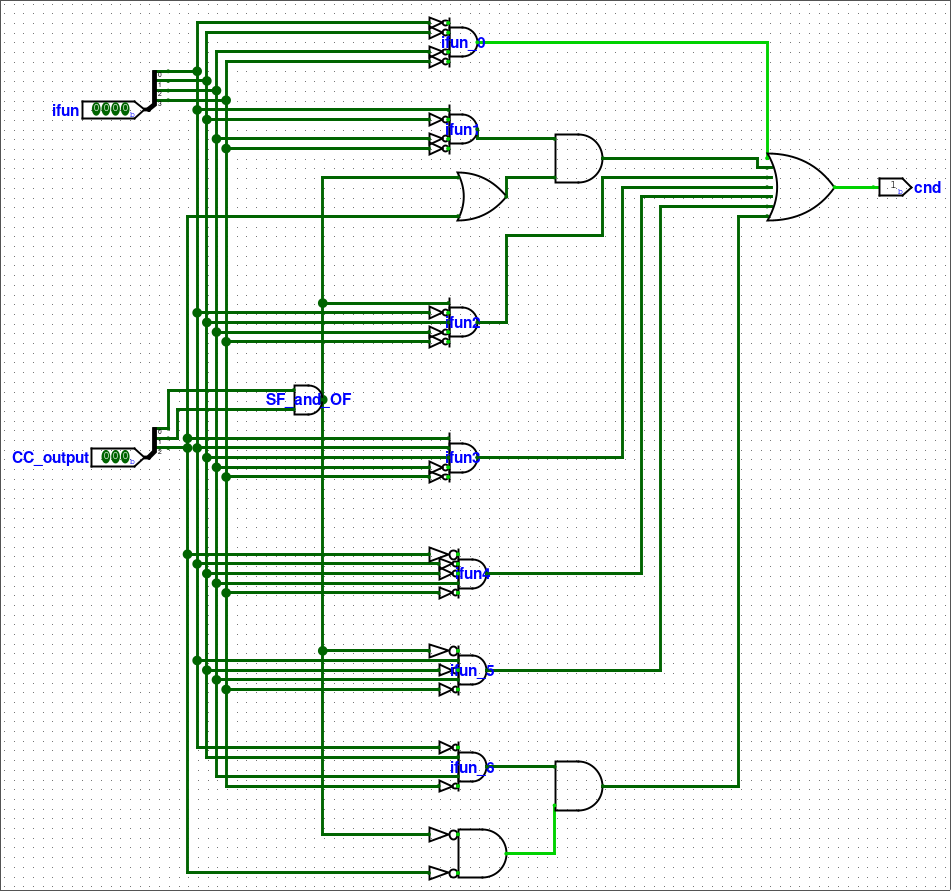
\includegraphics[width=0.8\textwidth]{./images/cond.png}
    \caption{Condition module}
\end{figure}

In the actual ALU module, both inputs go through a certain function determined by a 4x1 multiplexer that selects based on the ALU\_func module's output. 
The four possible functions are addition, subtraction, the bitwise AND operation, or the bitwise XOR operation. 
The condition code is determined by comparing the new value with 0. 
Overflow is also checked through the built-in adder operation. 

\begin{figure}[H]
    \centering
    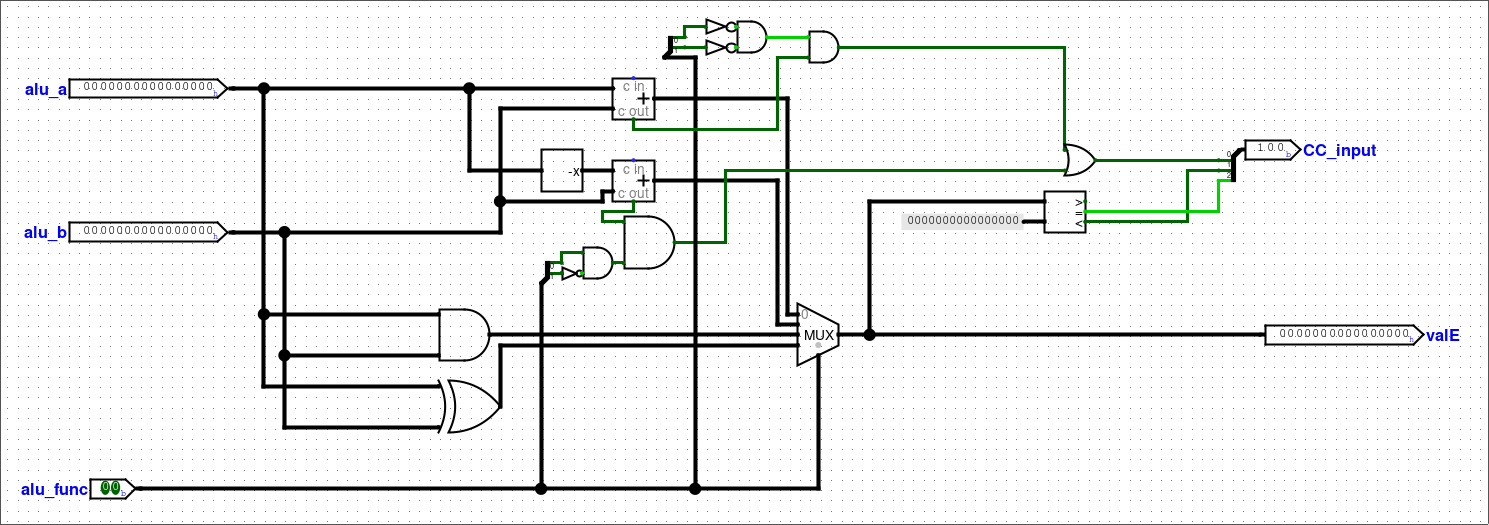
\includegraphics[width=0.8\textwidth]{./images/alu.png}
    \caption{ALU module}
\end{figure}

\subsection{Memory Stage}

The main function for the Memory stage is to read or write memory word. 
The control logic surrounding this stage is the stat, mem.read, mem.write, mem.addr, and the mem.data modules. 
The stat module concludes what the status of the instruction is. 
Mem.read determines if the word should be read. 
Likewise, Mem.write determines if the word should be written. 
Mem.addr selects the address and Mem.data selects the data. 

\begin{figure}[H]
    \centering
    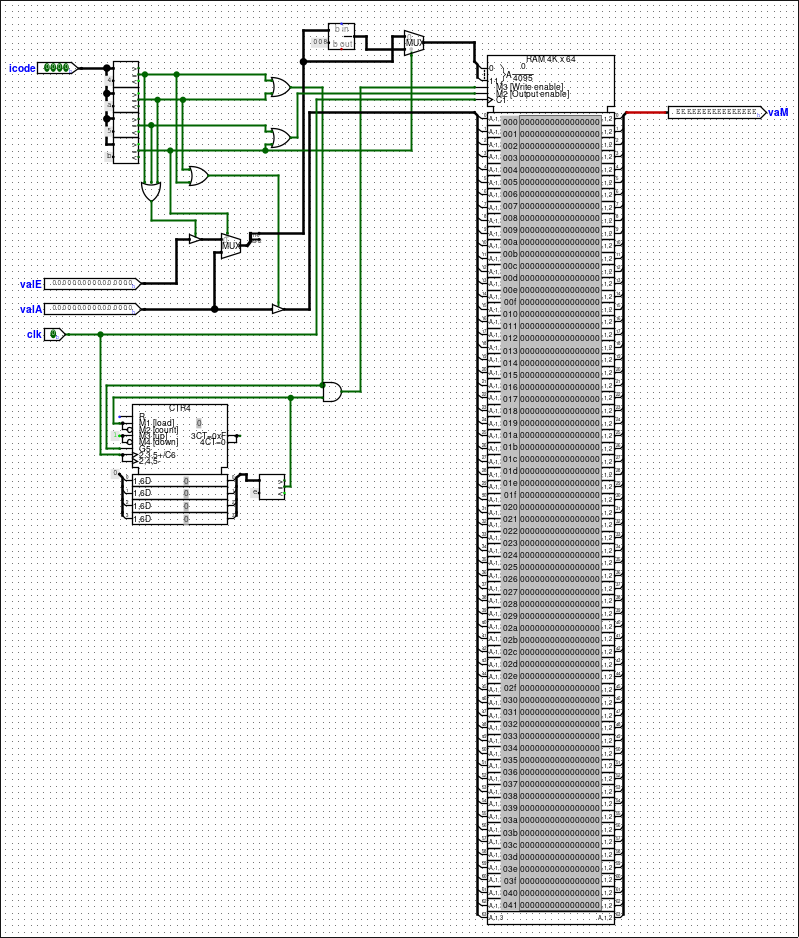
\includegraphics[width=0.8\textwidth]{./images/memory.png}
    \caption{Memory stage}
\end{figure}

\subsection{PC Update Stage}

The PC Update stage sets a new value for the program counter (PC). 
This new value is computed through a 16x1 multiplexer that is based on the instruction code. 
The multiplexer determines the current PC value and the result of certain operations or conditions within the processor. 
A special case is for instruction code 7 (any jump function) which uses a 2x1 multiplexer to determine the new PC between valC or valP, depending if the condition flag is on. 

\begin{figure}[H]
    \centering
    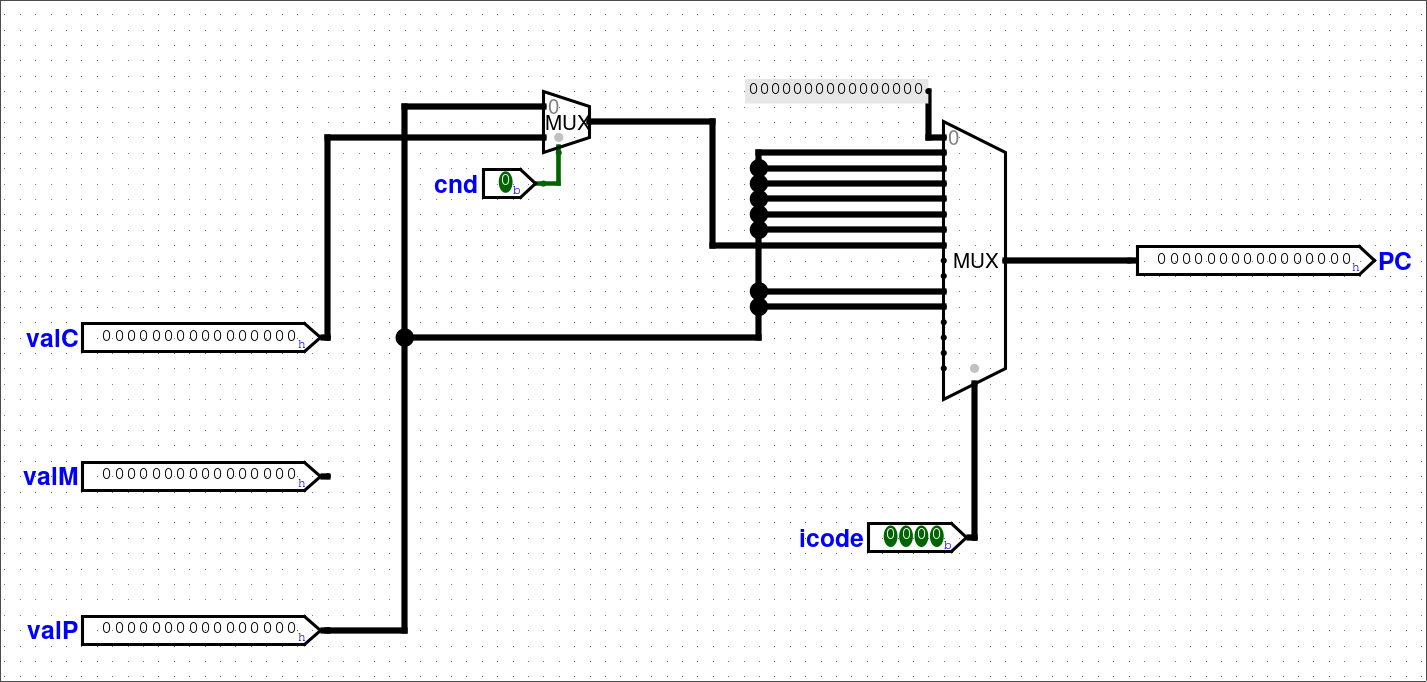
\includegraphics[width=0.8\textwidth]{./images/pc_update.png}
    \caption{PC Update stage}
\end{figure}

\section{Timing Analysis}

The following is a timing diagram for the Y86 ISA implementation.

\begin{figure}[H]
    \centering
    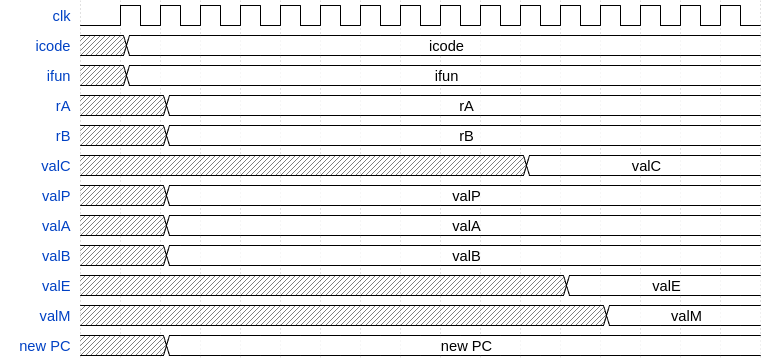
\includegraphics[width=\textwidth]{./images/wavedrom.png}
    \caption{Timing diagram for the Y86 ISA implementation}
\end{figure}

\section{Testing}

The following programs were used to test the correctness of the Y86 ISA implementation.

\subsection{Program 1}

\begin{lstlisting}[language=myassembly]
    .pos 0
    irmovq $100, %rsp
    irmovq $0xabc, %rax
    pushq %rax
    irmovq $0xdef, %rax
    pushq %rax
    irmovq $0xabcdeff, %rax
    popq %rcx
    popq %rdx
    rmmovq %rcx, 0x10
    mrmovq 0x10, %rdi
    jmp newpos
    nop
    nop
    rrmovq %rdi, %r11
newpos:
    rrmovq %rdi, %r12
    halt
\end{lstlisting}

This program verifies the following instructions:
\begin{itemize}
    \item irmovq
    \item pushq
    \item popq
    \item rmmovq
    \item mrmovq
    \item jmp
    \item nop
    \item rrmovq
    \item halt
\end{itemize}

The expected output is:

\begin{figure}[H]
    \centering
    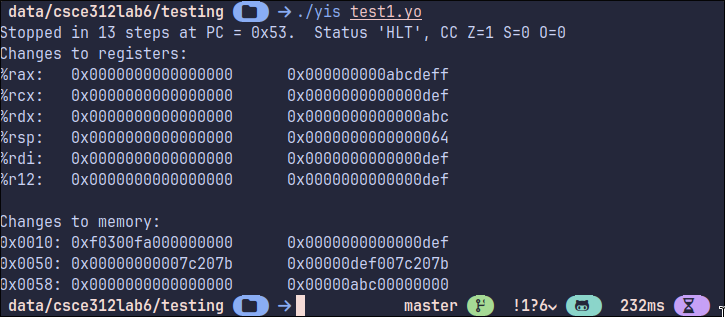
\includegraphics[width=0.8\textwidth]{./images/test1_out.png}
    \caption{Expected output for Program 1}
\end{figure}

The final values of the registers and memory are as follows:

\begin{minipage}{0.5\textwidth}
    \begin{figure}[H]
        \centering
        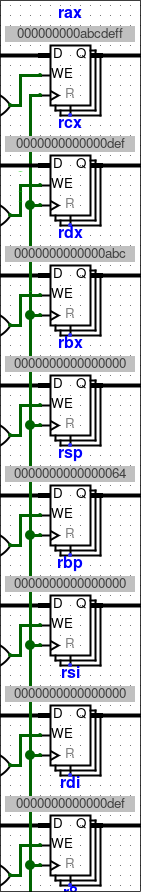
\includegraphics[width=0.5\textwidth]{./images/test1_reg1.png}
        \caption{Final register values for Program 1}
    \end{figure}
\end{minipage}
\begin{minipage}{0.5\textwidth}
    \begin{figure}[H]
        \centering
        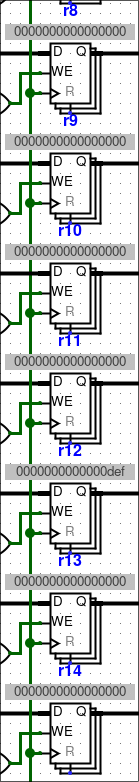
\includegraphics[width=0.5\textwidth]{./images/test1_reg2.png}
        \caption{Final register values for Program 1}
    \end{figure}
\end{minipage}

\begin{figure}
    \centering
    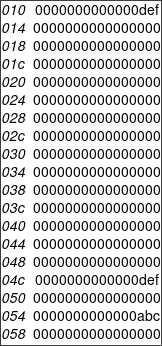
\includegraphics[width=0.5\textwidth]{./images/test1_mem.png}
    \caption{Final memory values for Program 1}
\end{figure}

\subsection{Program 2}

\begin{lstlisting}[language=myassembly]
    irmovq $0, %rax          # Load immediate 0 into %rax
    irmovq $10, %rbx         # Load immediate 10 into %rbx
    irmovq $1, %rcx          # Load immediate 1 into %rcx (loop counter)
    jmp loop

label:
    irmovq $20, %rdi
    jmp end

loop:
    addq %rbx, %rax          # Increment %rax by %rbx
    rrmovq %rax, %rdx        # Move %rax to %rdx

    irmovq $1, %rsi          # Load immediate 1 into %rsi
    subq %rsi, %rcx          # Decrement %rcx by 1
    irmovq $0, %rsi          # Reset %rsi to 0 for comparison

    # Use register value directly to control the loop: simple decrement and stop condition
    rrmovq %rcx, %rsi        # Copy %rcx to %rsi
    je label                 # Continue loop if %rcx is not equal to %rsi (i.e., not zero)

end:
    halt                     # Stop the program

\end{lstlisting}

This program verifies the following instructions:
\begin{itemize}
    \item irmovq
    \item addq
    \item rrmovq
    \item subq
    \item jne
    \item halt
\end{itemize}

The expected output is:

\begin{figure}[H]
    \centering
    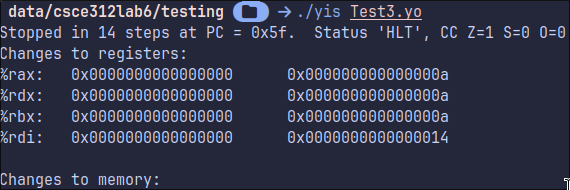
\includegraphics[width=0.8\textwidth]{./images/test3_out.png}
    \caption{Expected output for Program 2}
\end{figure}

The final values of the registers are as follows:

\begin{figure}
    \centering
    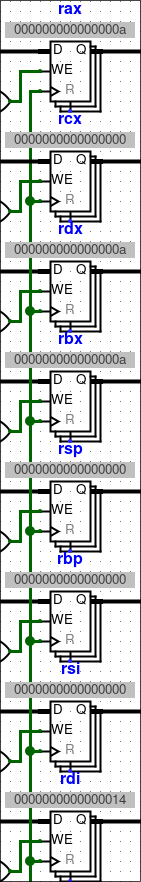
\includegraphics[width=0.2\textwidth]{./images/test3_reg.png}
    \caption{Final register values for Program 2}
\end{figure}

\subsection{Program 3}

\begin{lstlisting}[language=myassembly]
    # Initialize stack pointer
    irmovq $0x200, %rsp    
    
    # Initialize registers
    irmovq $10, %rax       # Load immediate 10 into %rax
    rmmovq %rax, 8(%rsp)  # Store %rax at memory address 8(%rsp)
    irmovq $5, %rdx        # Load immediate 5 into %rdx
    
    # Use memory and stack operations
    mrmovq 8(%rsp), %rbx  # Load %rbx from memory address 8(%rsp)
    pushq %rax             # Push %rax onto the stack
    pushq %rdx             # Push %rdx onto the stack as well
    
    # Perform arithmetic on the stack's top values
    popq %rcx              # Pop the top of the stack into %rcx (was %rdx)
    popq %rsi              # Pop the next top of the stack into %rsi (was %rax)
    addq %rsi, %rcx        # Add %rsi to %rcx, store the result in %rcx
    rrmovq %rcx, %rbx      # Move result back into %rbx for further use
    
    # More stack manipulations
    pushq %rbx             # Push the result back onto the stack
    pushq %rcx             # Push %rcx onto the stack again
    
    # Double the value at the top of the stack
    popq %rdi              # Pop the top of the stack into %rdi
    addq %rdi, %rdi        # Double the value in %rdi
    pushq %rdi             # Push the doubled value back onto the stack
    
    # Clean up and repeat operations
    nop                    # No operation
    halt                   # Stop the program
\end{lstlisting}

This program verifies the following instructions:
\begin{itemize}
    \item irmovq
    \item rmmovq
    \item mrmovq
    \item pushq
    \item popq
    \item addq
    \item rrmovq
    \item nop
    \item halt
\end{itemize}

The expected output is:

\begin{figure}[H]
    \centering
    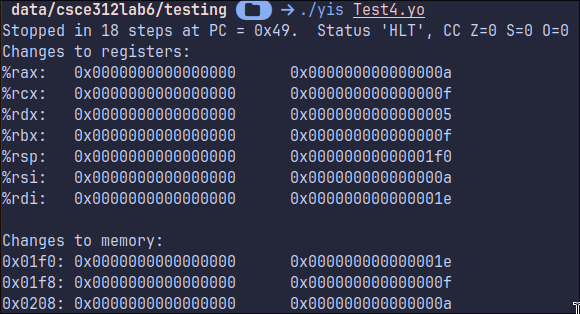
\includegraphics[width=0.8\textwidth]{./images/test4_out.png}
    \caption{Expected output for Program 3}
\end{figure}

The final values of the registers and memory are as follows:

\begin{minipage}{0.5\textwidth}
    \begin{figure}[H]
        \centering
        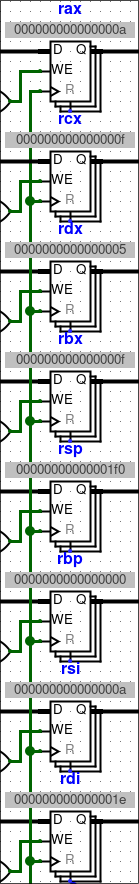
\includegraphics[width=0.4\textwidth]{./images/test4_reg.png}
        \caption{Final register values for Program 3}
    \end{figure}
\end{minipage}
\begin{minipage}{0.5\textwidth}
    \begin{figure}[H]
        \centering
        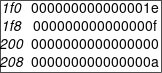
\includegraphics[width=0.5\textwidth]{./images/test4_mem.png}
        \caption{Final memory values for Program 3}
    \end{figure}
\end{minipage}


\end{document}
